\scanpage{81}
\mspage{329}

$3^\circ)$ On construit alors
\[
h_0=\xi^{-1}\ell_0^{\gamma}
\in\widehat{\Pi}_{0,3}
\]
La relation du $2^\circ)$ assure que $h_0\sigma_\infty(h_0)=1$ i.e.
que $h_0$ peut se mettre sous la forme
\[
h_0=\sigma_\infty(g_0)^{-1}g_0
\]
\unsure{avec} $g_0\in\widehat{\Pi}_{0,3}$.

\margin{NB Il faudrait s'assurer par contre que la connaissance de $g_0$
\unsure{ne} détermine pas $\gamma$ i.e. $p$
i.e. que \deleted{\illegible{2}} le $\gamma$
tel que $\xi=\ell_0^{\gamma}h_0^{-1}$
\unsure{satisfasse} (A) \unsure{ne} soit pas \deleted{\illegible{1}} unique.
À éclaircir!}

$4^\circ)$ On peut maintenant poser
\[
g=\sigma_\infty(g_0)\ell_1^{\gamma}\rho(g_0)^{-1}
=(g_0\ell_0^{-\gamma})\xi
\rho(g_0\ell_0^{-\gamma})^{-1}
\]
et on \deleted{\unsure{définit}} a ce qu'il faut pour définir $u$, via
\[
\left\{
\begin{aligned}
u(\sigma_\infty)&=\sigma_\infty\\
u(\rho)&=g\rho
\end{aligned}
\right.
\]

Ici, la seule équation délicate, \deleted{pour} laquelle
l'existence (non l'unicité, en bon cas) d'une solution, est problématique,
est l'équation C (en $\gamma\in\widehat{\mathbb Z}$)
--- plus la condition encore que $2\gamma+1\in\widehat{\mathbb Z}^{*}$.
C'est donc une \deleted{\unsure{question}}\inserted{\uline{condition}}
sur $\lambda\in\widehat{\Pi}_{0,3}$ --- ou plutôt deux types de condition,
suivant que $\xi$ est défini en termes de $\lambda$ par
l'une ou l'autre formule (B).

Je prévois qu'on est dans l'une ou

\margin{80}

\scanpage{82}

l'autre cas des formules (B), suivant que $p\bmod 3$ est congru à $1$, ou à $-1$
(NB. il ne doit pas être congru à $0$, puisque $p\bmod 3\in(\mathbb Z/3\mathbb Z)^*$)
i.e. suivant que $2\gamma\equiv 0$ ou $-2$ $(3)$ i.e.
$\gamma\equiv 0$ ou $-1$ $(3)$
(NB. il ne faut pas que $\gamma$ soit $\equiv 1$ $(3)$,
sinon $2\gamma+1=p$ serait congru à $0\bmod(3)$).
C'est en tous cas ce qui \unsure{sera} le cas si $u\in\Gamma_{\mathbb Q_0}$.

Pour le tester, réduisons le \deleted{\illegible{1}}\inserted{groupe}
$\widehat{\mathfrak S}_{0,3}^{+}$
mod l\deleted{es}\inserted{'}\unsure{équation|équations}
$\ell_0^3=1$ i.e. $(\sigma_\infty\rho)^6=1$
\[
\deleted{\ell_0^3=\ell_1^3=\ell_\infty^3=1\quad\ell_\infty}
\]
de sorte que $\widehat{\mathfrak S}_{0,3}^{+}$
est \unsure{remplacé} par une extension de $\mathfrak S_3$
par le groupe défini par les générateurs $\ell_0,\ell_1,\ell_\infty$ satisfaisant
\[
\unsure{\ell_0}^3=\ell_1^3=\ell_\infty^3=(\ell_\infty\ell_1\ell_0)=1
\]
--- ou mieux, utilisons
\[
\widehat{\mathfrak S}_{0,3}^{+}
\simeq\mathrm{Sl}(2,\mathbb Z)^{\prime\,\wedge}
\]
et réduisons carrément dans
\[
\mathrm{Sl}(2,\mathbb Z/6\mathbb Z)'
\simeq\mathrm{Sl}(2,\mathbb Z/2\mathbb Z)
\times\mathrm{Sl}(2,\mathbb Z/3\mathbb Z)'.
\]

\margin{81}

\scanpage{83}
\mspage{330}

Mais pour faire les calculs, il faut pouvoir identifier $\sigma_\infty$
\inserted{et} $\rho$ comme éléments de
$\mathrm{Sl}(2,\unsure{\widehat{\mathbb Z}|\mathbb Z})$
--- explicitation que nous ferons tantôt.

\begin{center}\rule{2cm}{0.4pt}\end{center}

Revenant à (24 bis), et y portant
$\unsure{h_0|h_\infty}=\xi^{-1}\ell_0^{\gamma}$, il vient
\[
\tag{61}
g_0=\widehat{\varphi}(\xi)
\varepsilon_0^{\gamma-\beta}
\]
On pense donc que $u$ correspond à
$(\xi,g_0,\gamma,\beta)$,
avec $\xi,g_0\in\widehat{\Pi}_{0,3}$
et $\gamma,\beta\in\widehat{\mathbb Z}$
\margin{\illegible{1}}
satisfaisant
\[
\tag{62}
\left\{
\begin{aligned}
&\xi\rho(\xi)\rho^2(\xi)=1\\
&\xi\underbrace{\sigma_\infty(g_0)^{-1}g_0}_{h}
=\ell_0^{\gamma}\\
&\deleted{\unsure{\widehat{\varphi}(\xi)}}g_0
=\widehat{\varphi}(\xi)
\varepsilon_0^{\gamma-\beta}\\
&2\gamma+1\in\widehat{\mathbb Z}^{*}
\end{aligned}
\right.
\]
dont on peut éliminer $g_0$, et on trouve des équations en
$(\xi,\deleted{\gamma}r,\deleted{\beta}s)$
$(r=\gamma-\beta,\ s=\gamma+\beta)$
\[
\tag{63}
\left\{
\begin{aligned}
&\xi\rho(\xi)\rho^2(\xi)=1\\
&\sigma_\infty\bigl(\widehat{\varphi}(\xi)\bigr)^{-1}
\widehat{\varphi}(\xi)
=\varepsilon_1^r\xi^{-1}\varepsilon_0^s\\
&\underbrace{r+s+1}_{p}\in\widehat{\mathbb Z}^{*}
\end{aligned}
\right.
\]
\margin{(donc $\xi=\lambda\rho(\lambda)^{-1}$
ou $\xi=\lambda\ell_0^{-1}\rho(\lambda)^{-1}$}

Ici, $\unsure{\lambda}$ est déterminé mod transformation en
$\lambda'=\deleted{\unsure{\ell_0^{\alpha}\xi}}\ell_0^\alpha\lambda$
donc $\xi$ devient
$\xi'=\ell_0^\alpha\xi\ell_1^{-\alpha}$

\margin{82}

\scanpage{84}
\mspage{331}

\uline{42} Récapitulation sur le groupe
\[
(\mathfrak S_{0,3})
\simeq
\bigl(\Pi_1(U_{0,3}^{\mathrm{an}},\mathfrak S_3;-\bar j)\bigr)
\simeq
\bigl(\widetilde\Pi'_{0,3}\simeq
\Pi_1((\mathbb P^{1\mathrm{an}},0\{0\}+2\{1\}+3\{\infty\}),\unsure{\{1,\tau\}};-\bar j)\bigr)
\]
\[
\simeq\bigl(\mathrm{Gl}(2,\mathbb Z)'=\mathrm{Gl}(2,\mathbb Z)/\{\pm1\}
\simeq\mathrm{GP}(1,\mathbb Z)\bigr)
\simeq\bigl(\mathcal T'_{1,1}=\mathcal T_{1,1}/\{\pm1\}\bigr)
\]
et sur les automorphismes ``de lacets'' de
$\widehat{\mathfrak S}_{0,3}^{+}$ et de
$\widehat\Pi_{0,3}$ (Formulaire fondamental).

\margin{\deleted{\illegible{1}} $\mathfrak S_{0,3}$ défini comme $\mathrm{Aut}_{\mathrm{lac}}(\Pi_{0,3})$ --- on en donne \uline{cinq} \unsure{visions} différentes ! (En fait, il y en a \uline{une} dizaine, cf. (V) ci-dessous\ldots)}

\uline{I}) $\mathcal T_{0,3}$

Le groupe $\mathfrak S_{0,3}$ est \unsure{présenté} comme une extension
\[
(1)\qquad
\diagram{\begin{tikzcd}[ampersand replacement=\&,column sep=small]
1 \arrow[r,dash] \& \Pi_{0,3} \arrow[r] \arrow[d,phantom,"\Vert"] \& \mathfrak S_{0,3} \arrow[r] \& \mathcal T_{0,3} \arrow[r] \arrow[d,phantom,"\wr"] \& 1 \\
\& \Pi_1(U_{0,3}^{\mathrm{an}};-\bar j) \&\& \mathfrak S_3\times\mathbb Z/2\mathbb Z \&
\end{tikzcd}}
\]
où $\mathfrak S_3\times\mathbb Z/2\mathbb Z$ est considéré comme groupe opérant sur
$U_{0,3}^{\mathrm{an}}=\mathbb P^{1\mathrm{an}}\setminus\{0,1,\infty\}=\mathbb C\setminus\{0,1\}$,
\deleted{par \unsure{autom.} holomorphes}
\deleted{$\mathfrak S_3$ opérant par permutations}
--- c'est le groupe des automorphismes conformes \unsure{du|de} $\mathbb P^{1\mathrm{an}}$ qui stabilisent $\{0,1,\infty\}$.
Le groupe \margin{\unsure{(2)}}\deleted{\unsure{$\mathfrak S_3$}}\inserted{$\mathfrak S_3=\mathfrak S_{\{0,1,\infty\}}$} est le sous-groupe des \deleted{\unsure{éléments}}automorphismes conformes, il s'identifie au groupe des permutations de $\{0,1,\infty\}$, ses six éléments sont
\unsure{$\mathrm{id}$;|$1$;}
$\dot\sigma_0,\dot\sigma_1,\dot\sigma_\infty$ (\inserted{les trois} transpositions),
$\dot\rho,\deleted{\unsure{\dot{\rho}}}\dot\rho^{-1}$ (permutations circulaires)
donnés par les formules explicites
\[
(2)\qquad
\left\{\begin{array}{l}
\dot\sigma_0(z)=\dfrac{z}{z-1}\inserted{\unsure{=1+\dfrac{1}{1-z}|=1+\dfrac{1}{z-1}}},\quad
\dot\sigma_1(z)=\dfrac1z,\quad
\dot\sigma_\infty(z)=1-z,\\[4pt]
\dot\rho(z)=\dfrac1{1-z},\quad
\dot\rho^{-1}(z)=1-\dfrac1z=\dfrac{z-1}{z},
\end{array}\right.
\]
avec
\[
(3)\qquad
\left\{\begin{array}{l}
\dot\sigma_0\dot\sigma_1=\dot\sigma_1\dot\sigma_\infty=\dot\sigma_\infty\dot\sigma_0=\dot\rho,\\
\dot\rho\dot\sigma_0\dot\rho^{-1}=\dot\sigma_1,\quad
\dot\rho\dot\sigma_1\dot\rho^{-1}=\dot\sigma_\infty,\quad
\dot\rho\dot\sigma_\infty\dot\rho^{-1}=\dot\sigma_0
\end{array}\right.
\]
\[
(4)\qquad
\dot\sigma_0^2=\dot\sigma_1^2=\dot\sigma_\infty^2=\dot\rho^3=1.
\]
Le groupe $\mathcal T'_{0,3}=\mathbb Z/2\mathbb Z\subset\mathcal T_{0,3}$ apparaît comme le centre,
\margin{83}

\scanpage{85}

il est engendré par la conjugaison complexe $\tau$
\[
(5)\qquad ,\quad \tau(z)=\bar z,
\]
les cinq autres éléments de $\mathcal T_{0,3}$ sont
\[
\deleted{\unsure{\tau\sigma}}\quad(6)\qquad
\tau\dot\sigma_0=\dot\tau_0,\quad
\tau\dot\sigma_1=\dot\tau_1,\quad
\tau\dot\sigma_\infty=\dot\tau_\infty,\quad
\tau\rho,\quad\tau\rho^{-1}=(\tau\rho)^{-1},
\]
les \unsure{antiinvolutions|anti-involutions} $\tau'_i$ $(i=0,1,\infty)$ sont particulièrement intéressantes, \unsure{données} par
\[
(7)\qquad
\unsure{\dot\tau'_0(z)}=\frac{\bar z}{\bar z-1},\quad
\unsure{\dot\tau'_1(z)}=\frac1{\bar z},\quad
\dot\tau'_\infty(z)=1-\bar z.
\]

Les points fixes \deleted{\unsure{dans $U_{0,3}$}} des \inserted{\illegible{1}} autom. conformes de \deleted{\illegible{2}} $(\mathbb P^{1\mathrm{an}},\{0,1,\infty\})$ sont les suivants
\[
\begin{gathered}
(8)\qquad
\left\{\begin{array}{l}
(\mathbb P^1_{\mathbb C})^{\dot\sigma_0}=\{0,2\},\\[3pt]
(\mathbb P^1_{\mathbb C})^{\dot\sigma_1}=\{1,-1\},\\[3pt]
(\mathbb P^1_{\mathbb C})^{\dot\sigma_\infty}=\{\infty,\frac12\}\\[3pt]
\mathbb P_{\mathbb C}^{1\,\dot\rho}=\mathbb P^{1\,\dot\rho^{-1}}=\{-\bar j,-j\}
\end{array}\right.\\[6pt]
\begin{array}{l}
\text{où }j=\exp 2i\pi/3=\dfrac{-1+i\sqrt3}{2}\quad\text{racine primitive}\quad\text{$3^{\unsure{\mathrm{ième}|\mathrm{ème}}}$ de $1$}\\[5pt]
-\bar j=\exp 2i\pi/6=\dfrac{1+i\sqrt3}{2}\quad\text{racine primitive}\quad\text{$6^{\unsure{\mathrm{ième}|\mathrm{ème}}}$ de $1$}
\end{array}\end{gathered}
\]

\margin{NB $\mathbb P_{\mathbb C}^{1\,\dot\rho\tau}=\mathbb P_{\mathbb C}^{1\,\dot\rho^{-1}\tau}=\varnothing$}

\[
(9)\qquad
\left\{\begin{array}{l}
\mathbb P_{\mathbb C}^{1\,\tau}=\mathbb P_{\mathbb R}^{1}\\[3pt]
\mathbb P_{\mathbb C}^{1\,\dot\tau'_0}=\{x+iy\mid(x-1)^2+y^2=1\}\\[-1pt]
\quad\inserted{=\{z\mid z+\bar z=z\bar z\}\unsure{=\frac1z|=\frac12}}
\inserted{\unsure{=\frac12-\mathbb U}},\\[3pt]
\mathbb P_{\mathbb C}^{1\,\dot\tau'_1}=\{z\mid z\bar z=1\}=\{x+iy\mid x^2+y^2=1\}=\mathbb U\\[3pt]
\mathbb P_{\mathbb C}^{1\,\dot\tau'_\infty}=\{z\mid z+\bar z=1\}=\{x+iy\mid x=\frac12\}=\frac12+i\mathbb R;
\end{array}\right.
\]

L'image la plus suggestive est sans doute celle de la sphère de Riemann, où $\tau,\dot\tau'_0,\dot\tau'_1,\dot\tau'_\infty$ apparaissent comme les \deleted{\unsure{symétries}}\inserted{\uline{réflexions}} p.r. aux \deleted{``équateurs''}\inserted{``\unsure{gr\textsuperscript{ds}|grands} cercles''} correspondants, qui pour $\tau$ est ``l'équateur'' et pour les autres sont les grands cercles \inserted{``méridiens''}, passant par les pôles $-\bar j,-j$, qui réalisent le découpage de l'équateur en six segments circulaires, par les pts de subdivision $0,\frac12,1,2,\infty,-1$.

\figure{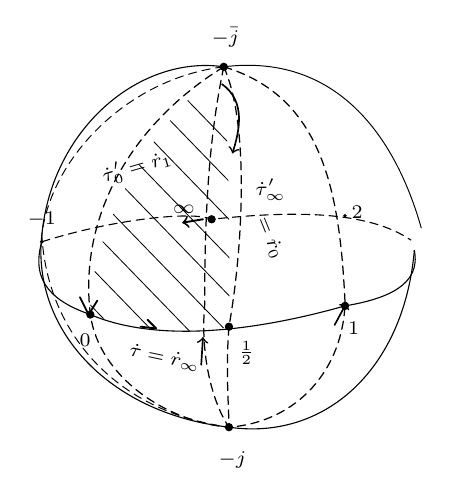
\begin{tikzpicture}[x=.022cm,y=-.022cm,line cap=round,line join=round,font=\scriptsize]
\coordinate (N) at (110,8);
\coordinate (S) at (113,216);
\draw[line width=.4pt] (N) .. controls (62,1) and (11,43) .. (5,105)
 .. controls (-1,158) and (42,208) .. (S)
 .. controls (168,224) and (214,183) .. (220,114);
\draw[line width=.35pt] (N) .. controls (175,0) and (209,48) .. (224,101);
\begin{scope}
\clip (N) .. controls (62,47) and (32,109) .. (33,151)
 .. controls (60,160) and (91,164) .. (113,158)
 .. controls (114,100) and (112,43) .. (N);
\foreach \a in {-80,-58,-36,-14,8,30,52,74,96,118,140,162}
  \draw[line width=.3pt] (-15,\a)--(145,{\a+165});
\end{scope}
\draw[dash pattern=on 3pt off 2pt,line width=.45pt] (N)
 .. controls (58,40) and (26,93) .. (33,151)
 .. controls (38,187) and (77,213) .. (S);
\draw[dash pattern=on 3pt off 2pt,line width=.45pt] (N)
 .. controls (101,51) and (99,95) .. (99,145)
 .. controls (96,180) and (106,206) .. (S);
\draw[dash pattern=on 3pt off 2pt,line width=.45pt] (N)
 .. controls (125,41) and (121,113) .. (113,158)
 .. controls (111,183) and (113,205) .. (S);
\draw[dash pattern=on 3pt off 2pt,line width=.45pt] (N)
 .. controls (167,25) and (177,80) .. (180,144)
 .. controls (179,182) and (153,213) .. (S);
\draw[dash pattern=on 3pt off 2pt,line width=.35pt] (N)
 .. controls (53,15) and (10,62) .. (5,105)
 .. controls (8,161) and (47,207) .. (S);
\draw[dash pattern=on 3pt off 2pt,line width=.4pt] (5,109)
 .. controls (46,96) and (92,91) .. (103,96)
 .. controls (150,91) and (193,91) .. (218,108);
\draw[line width=.4pt] (5,109) .. controls (-2,133) and (13,144) .. (33,151)
 .. controls (80,171) and (148,155) .. (180,146)
 .. controls (204,142) and (224,134) .. (220,114);
\draw[->,line width=.7pt] (98,96)--(86,98);
\draw[->,line width=.6pt] (109,18) .. controls (123,28) and (119,45) .. (115,58);
\draw[->,line width=.6pt] (97,180)--(98,164);
\draw[->,line width=.6pt] (174,157)--(181,144);
\draw[line width=.65pt] (27,141)--(32,151)--(37,143);
\draw[line width=.65pt] (62,158)--(71,159)--(66,154);
\foreach \p in {(110,8),(113,216),(103,96),(33,151),(113,158),(180,146)}
  \fill \p circle[radius=2.4];
\foreach \p in {(5,109),(180,94)}
  \fill \p circle[radius=1.1];
\node[inner sep=0pt] at (111,-9) {$-\bar j$};
\node[inner sep=0pt] at (115,235) {$-j$};
\node[inner sep=0pt] at (5,96) {$-1$};
\node[inner sep=0pt] at (87,90) {$\infty$};
\node[inner sep=0pt] at (187,92) {$2$};
\node[inner sep=0pt] at (30,166) {$0$};
\node[inner sep=0pt] at (123,173) {$\frac12$};
\node[inner sep=0pt] at (185,159) {$1$};
\node[inner sep=0pt,rotate=16] at (60,66) {$\dot\tau'_0=\dot r_1$};
\node[inner sep=0pt] at (137,79) {$\dot\tau'_\infty$};
\node[inner sep=0pt,rotate=-68] at (137,107) {$=\dot r_0$};
\node[inner sep=0pt,rotate=-12] at (76,176) {$\unsure{\dot\tau}=\unsure{\dot r}_\infty$};
\end{tikzpicture}}

Notons aussi les formules
\[
(10)\qquad
\left\{\begin{array}{l}
\dot\rho\dot\tau'_0\dot\rho^{-1}=\dot\tau'_1,\quad
\dot\rho\dot\tau'_1\dot\rho^{-1}=\dot\tau'_\infty,\quad
\dot\rho\dot\tau'_\infty\dot\rho^{-1}=\dot\tau'_0\\[3pt]
\dot\tau'_0\dot\tau'_1=\dot\tau'_1\dot\tau'_\infty=\dot\tau'_\infty\dot\tau'_0=\dot\rho
\end{array}\right.
\]
\margin{84}

\scanpage{86}
\mspage{332}

Les quatre grands cercles (9) découpent la sphère en 12 triangles sphériques, qui forment des domaines fondamentaux pour le groupe $\mathcal T_{0,3}\simeq\mathfrak S_3\times\mathbb Z/2$ d'ordre 12, et sont permutés entre eux de façon simplement transitive.
\deleted{\unsure{Prenant|Prenons} un de}\inserted{(C'est \unsure{aussi|ainsi}} la subdivision barycentrique des doubles triangles sphériques \unsure{déterminés} par l'équateur $\mathbb P_{\mathbb R}^{1}$, et ses trois pts de subdivision $0,1,\infty$.)
Prenons un de ces triangles sphériques, disons $(-\bar j,0,\frac12)$, les réflexions p.r. à ses \inserted{trois} côtés, i.e.
$\tau,\dot\tau'_\infty,\dot\tau'_0$, forment un syst. de générateurs de $\mathcal T_{0,3}$, avec les relations
\[
(11)\qquad
\tau^2=\dot\tau_\infty^{\prime 2}=\dot\tau_0^{\prime 2}
=\left(\underbrace{\unsure{\tau}\dot\tau'_\infty\tau}_{\dot\sigma_\infty}\right)^2
=\left(\underbrace{\dot\tau'_0\dot\tau'_\infty}_{\dot\rho^{-1}}\right)^3
=\left(\underbrace{\tau\unsure{\dot\tau'_0}\deleted{\unsure{\tau}}}_{\dot\sigma_0}\right)^2=1
\]

quant à $\mathfrak S_3=\mathcal T_{0,3}^{+}$, il est engendré par
$\tau\dot\tau'_\infty=\dot\sigma_\infty$, $\dot\tau'_0\dot\tau'_\infty=\dot\rho^{\unsure{-1|1}}$ et $\tau\dot\tau'_0=\dot\sigma_0$, avec les relations
\[
(12)\qquad
\dot\sigma_0\dot\rho\dot\sigma_\infty=\dot\sigma^2=\dot\rho^3=\dot\sigma_0^2=1.
\]

\uline{II}) Le groupe $\Pi_{0,3}$ est engendré par $\ell_0,\ell_1,\ell_\infty$, liés par la relation génératrice
\[
(13)\qquad \ell_\infty \ell_1\ell_0=1
\]
Le \deleted{groupe} sous-groupe \inserted{d'indice 2}
$\mathfrak S'_3=(\mathcal T_{0,3})_{-\bar j}=\unsure{\mathcal T_{0,3}}$,
stabilisateur de $-\bar j$, formé des $(g,\tau^\varepsilon)\in\mathfrak S_3\times\mathbb Z/2\mathbb Z$ tels que $\mathrm{sg}(g)=(-1)^\varepsilon$, opère sur $\Pi_{0,3}$.
Ce sous-groupe est formé de $1,\dot\tau_0,\dot\tau_1,\dot\tau_\infty,\dot\rho,\dot\rho^{-1}$, et leurs opérations sur $\Pi_{0,3}$ sont notées respectivement $1,\tau'_0,\tau'_1,\tau'_\infty,\rho,\rho^{-1}$.

\margin{\uline{NB} $\tau'_0,\tau'_1,\tau'_\infty$ étaient notés précédemment (dans [C]) $\unsure{\sigma_0,\sigma_1,\sigma_\infty|\bar\sigma_0,\bar\sigma_1,\bar\sigma_\infty}$.}
\margin{85}

\scanpage{87}

\deleted{(14)}\quad\deleted{$\rho(\ell_0)=$}
On identifie ces éléments \deleted{aux} \inserted{à des éléments du} groupe
$\mathrm{Aut}_{\mathrm{lac}}(\Pi_{0,3})\simeq\mathfrak S_{0,3}$,
\deleted{\illegible{3} $\mathfrak S_{0,3}$ \illegible{1}}
donc \deleted{\illegible{1}} pour $g\in\mathfrak S'_3$, $x\in\Pi_{0,3}$, on pose
$g(x)=gxg^{-1}$; et on trouve :
\[
\tag{14}
\left\{\begin{aligned}
\rho(\ell_0)&=\rho\ell_0\rho^{-1}=\ell_1,&
\rho(\ell_1)&=\rho\ell_1\rho^{-1}=\ell_\infty,&
\rho(\ell_\infty)&=\rho\ell_\infty\rho^{-1}=\ell_0,\\
\unsure{\dot\tau'_0|\tau'_0}(\ell_0)&=\ell_0^{-1},&
\unsure{\dot\tau'_0|\tau'_0}(\ell_1)&=\ell_\infty^{-1},&
\unsure{\dot\tau'_0|\tau'_0}(\ell_\infty)&=\ell_1^{-1},\\
\tau'_1(\ell_1)&=\ell_1^{-1},&
\tau'_1(\ell_\infty)&=\ell_0^{-1},&
\tau'_1(\ell_0)&=\ell_\infty^{-1},\\
\tau'_\infty(\ell_\infty)&=\ell_\infty^{-1},&
\tau'_\infty(\ell_0)&=\ell_1^{-1},&
\tau'_\infty(\unsure{\ell_0|\ell_1|\ell_\infty})&=\ell_1^{-1}
\end{aligned}\right.
\]
\[
\tag{15}
:\quad\tau'_0\tau'_1=\tau'_1\tau'_\infty=\tau'_\infty\tau'_0=\rho
\qquad\text{(et bien sûr \inserted{on a} }{\tau'_0}^{2}={\tau'_1}^{2}=\unsure{{\tau'_\infty}^{2}|\tau_\infty^{2}}=\rho^3=1\text{).}
\]

\inserted{Dans} Le groupe $\mathfrak S_{0,3}$ on \unsure{définit} des éléments
$\sigma_0,\sigma_1,\sigma_\infty$, au dessus de $\dot\sigma_0,\dot\sigma_1,\dot\sigma_\infty$, par
\[
\tag{16}
\left\{\begin{aligned}
\sigma_0(\ell_1)&=\ell_\infty,& \sigma_0(\ell_\infty)&=\ell_1,& \sigma_0(\ell_0)&=(\ell_1\ell_\infty)^{-1}\\
\sigma_1(\ell_\infty)&=\ell_0,& \sigma_1(\ell_0)&=\ell_\infty,& \sigma_1(\ell_1)&=(\ell_\infty\ell_0)^{-1}\\
\sigma_\infty(\ell_0)&=\unsure{\ell_1},& \sigma_\infty(\unsure{\ell_1})&=\ell_0,& \sigma_\infty(\ell_\infty)&=(\ell_0\ell_1)^{-1}
\end{aligned}\right.
\]

On a
\[
\tag{17}
\left\{\begin{aligned}
\rho\sigma_0\rho^{-1}&=\sigma_1,& \rho\sigma_1\rho^{-1}&=\sigma_\infty,& \rho\sigma_\infty\rho^{-1}&=\sigma_0\\
\rho\tau_0\rho^{-1}&=\tau_1,& \rho\tau_1\rho^{-1}&=\tau_\infty,& \rho\tau_\infty\rho^{-1}&=\tau_0
\end{aligned}\right.,
\]
\[
\tag{18}
\sigma_0\sigma_1=\rho\ell_0=\deleted{\unsure{\rho}}\unsure{\ell_1\rho},\quad
\sigma_1\sigma_\infty=\rho\ell_1=\ell_\infty\rho,\quad
\sigma_\infty\sigma_0=\rho\ell_\infty=\ell_0\rho^{-1}.
\]

\margin{NB $\sigma_0,\sigma_1,\sigma_\infty\in\mathfrak S_{0,3}^{+}$,
$\tau'_0,\tau'_1,\tau'_\infty\in\mathfrak S_{0,3}^{-}$,
$\tau_0,\tau_1,\tau_\infty\in\mathfrak S_{0,3}^{-}$.}

On a ainsi des éléments de $\mathfrak S_{0,3}$ au dessus \unsure{de|des}
$1,\dot\sigma_0,\dot\sigma_1,\dot\sigma_\infty,\dot\rho,\dot\rho^{-1},\dot\tau'_0,\dot\tau'_1,\dot\tau'_\infty$,
mais pas encore au dessus de $\tau$ (ce qui permet d'en avoir sur $\tau\dot\rho,\tau\dot\rho^{-1}$),
on pose
$\tau_i=\underbrace{\sigma_i}_{\text{sur }\dot\sigma_i}\underbrace{\tau'_i}_{\text{sur }\dot\tau'_i}$
\inserted{$=\tau'_i\sigma_i$}
(qui est sur $\tau$, \deleted{donc}
\deleted{\illegible{1} $\in\mathfrak S_{0,3}$}
\uline{$\tau_i$ est \unsure{caractérisé}} \deleted{\illegible{1}}
par la condition d'être sur $\tau$, \inserted{\unsure{de carré $1$,}} et de commuter à $\sigma_i$ (ou encore, à $\tau'_i$)
\margin{\unsure{rappeler pourquoi on a cette} \uline{\unsure{caractérisation}}.}
\[
\tag{19}
[\tau_0,\sigma_0]=[\tau_1,\sigma_1]=[\tau_\infty,\sigma_\infty]=1
\]
\margin{$\begin{aligned}
\tau_0&=\sigma_0\tau'_0&\tau_1&=\sigma_1\tau'_1&\tau_\infty&=\sigma_\infty\tau'_\infty\\
&=\tau'_0\sigma_0&&=\tau'_1\sigma_1&&=\tau'_\infty\sigma_\infty
\end{aligned}$}
\[
\tag{20}
\tau_0^2=\tau_1^2=\tau_\infty^2=1
\qquad\text{et }\tau_0,\tau_1,\tau_\infty\text{ sur }\tau.
\]
On trouve
\[
\tag{21}
\tau_\infty\tau_1=\ell_0,\quad\tau_0\tau_\infty=\ell_1,\quad\tau_1\tau_0=\ell_\infty.
\]
Pour bien faire, il faudrait expliciter la description \unsure{topologique} (faite dans [C]) de
$\sigma_0,\sigma_1,\sigma_\infty,\rho,\tau'_0,\tau'_1,\tau'_\infty,\tau_0,\tau_1,\tau_\infty$.

\margin{86}

\scanpage{88}
\mspage{333}

On a
\[
\tag{22}
\left\{\begin{aligned}
(\sigma_\infty\rho)^2&=(\rho\sigma_1)^2=\ell_0=\varepsilon_0^2,&
\varepsilon_0&\overset{\unsure{\text{dfn}|\text{déf}}}{=}\sigma_\infty\rho=\rho\sigma_1\deleted{\unsure{\overset{\mathrm{dfn}}{=}}}
\\[-1pt]&&&\quad(\mathrm{NB}\ \sigma_\infty=\rho\sigma_1\rho^{-1})\\
(\sigma_0\rho)^2&=(\rho\sigma_\infty)^2=\ell_1=\varepsilon_1^2,&
\varepsilon_1&=\unsure{\sigma_0}\rho=\rho\sigma_\infty\\
(\sigma_1\rho)^2&=(\rho\unsure{\sigma_\infty|\sigma_0})^2=\ell_\infty=\varepsilon_\infty^2,&
\varepsilon_\infty&=\sigma_1\rho=\rho\sigma_0
\end{aligned}\right.
\]

L'élément $\varepsilon_i\in\mathfrak S_{0,3}$
(en fait $\varepsilon_i\in\mathfrak S_{0,3}^{+}$) est au dessus de $\dot\sigma_i$,
il est \uline{caractérisé} par la condition
\[
\varepsilon_i^2=\ell_i.
\]

Dans le groupe $\mathcal T_{0,3}$ d'ordre $12$, il y a sept éléments \unsure{involutifs}
$\dot\sigma_0,\dot\sigma_1,\dot\sigma_\infty,\tau,\dot\tau'_0,\dot\tau'_1,\dot\tau'_\infty$,
\deleted{et \unsure{quatre}} \inserted{deux} éléments d'ordre $3$
$\dot\rho,\dot\rho^{-1}$, \inserted{et \uline{deux d'ordre $6$}}
$\dot\rho\tau,\dot\rho^{-1}\tau$ (en plus de l'unité).

\inserted{Sauf les deux derniers (pour lesquels ce n'est pas possible$^*$)}
Nous \unsure{avons} \unsure{relevé} chacun de ces éléments en des éléments de $\overline{\mathrm m}$ ordre de
$\mathfrak S_{0,3}$.
\margin{$^*$ en effet ${\mathbb P^1}^{\dot\rho\tau}={\mathbb P^1}^{\dot\rho^{-1}\tau}=\varnothing$}
On sait que les possibilités, mod $\Pi_{0,3}$-conjugaison, \unsure{de|des} tels relèvements,
correspondent aux composantes connexes des pts fixes \unsure{dans|de} $U=U_{0,3}^{\mathrm{an}}$
des autom. \unsure{topologiques} correspondants. --- pour
$\dot\sigma_0,\dot\sigma_1,\dot\sigma_\infty,\dot\tau'_0,\dot\tau'_1,\dot\tau'_\infty$
il n'y a qu'une possibilité mod conjugaison (on a choisi
$\sigma_0,\sigma_1,\sigma_\infty,\tau_0,\tau_1,\tau_\infty$
de la façon qui a semblé le plus commode pour les calculs),
pour $\tau$ il y en a trois --- ce sont les trois choix $\tau_0,\tau_1,\tau_\infty$
--- pour $\dot\rho,\dot\rho^{-1}$ il y en a deux,
\unsure{correspondants|correspondantes} aux deux pôles $-\bar j,-j$ --- nous avons choisi celle qui
correspond au pôle $-\bar j$.
Les relèvements correspondants à $-j$ \unsure{peuvent} s'en déduire en \unsure{conjuguant} par un $\tau_i$ :

\margin{87}

\scanpage{89}

\[
(23)\quad
\begin{gathered}
\rho_0=\tau_0\rho\tau_0^{-1}
\inserted{=\ell_\infty^{-1}\rho=\unsure{\rho \ell_1^{-1}}},\qquad
\rho_1=\tau_1\rho\tau_1^{-1}
\inserted{=\ell_0^{-1}\rho=\rho \ell_\infty^{-1}},\\
\rho_\infty=\tau_\infty\rho\unsure{\tau_\infty^{-1}}
\inserted{=\ell_1^{-1}\rho=\rho \ell_0^{-1}}
\end{gathered}
\]
sont d'ordre 3, au dessus de $\dot\rho$, et $\Pi_{0,3}$-conjugués entre eux\textsuperscript{*}, mais non $\Pi_{0,3}$-conjugués à $\rho$.

\margin{* NB
\[
\begin{gathered}
\rho\rho_0\rho^{-1}=\rho_1\\
\rho\rho_1\rho^{-1}=\rho_\infty\\
\rho\rho_\infty\rho^{-1}=\rho_0
\end{gathered}
\]}

Notons aussi \deleted{que les} les formules \unsure{corollaires} de la théorie générale -- et du fait que les composantes conn. des ens. des pts fixes qui apparaissent ici sont 1-connexes --
\[
(24)\qquad
\Pi_{0,3}^{\sigma_i}=\Pi_{0,3}^{\rho}
=\Pi_{0,3}^{\tau_i}=\Pi_{0,3}^{\tau_i'}=\{1\}
\]

Si on regarde les pts critiques de $U_{0,3}^{\mathrm{an}}$, \unsure{relatifs} à l'opération de $\mathcal{T}_{0,3}$, on trouve les \deleted{\unsure{pts}\ \illegible{1}}\inserted{deux orbites} $(2,-1,\frac12)$ et $(-\bar j,-j)$, le stabilisateur d'un point de ces orbites est d'ordre 4 resp. 6.
Pour le pt 2 (opposé à 0), ce stabilisateur est le groupe $\mathrm{D}_2\simeq\mathbb{Z}/2\mathbb{Z}\times\mathbb{Z}/2\mathbb{Z}$, engendré par $\dot\sigma_0,\dot\tau_0$ (ou $\sigma_0,\tau_0'$) -- qui a été bel et bien relevé multiplicativement dans $\mathfrak S_{0,3}$.
De $\unsure{\overline{\mathrm m}|=}$, pour le point $-\bar j$, c'est $\mathfrak S_3'\inserted{\simeq\mathrm{D}_3}$, qui a été relevé également.
Par la théorie générale on sait que les classes de $\Pi_{0,3}$-conjugaison d'un tel relèvement correspondent aux pts fixes du groupe d'opérateurs \inserted{envisagé} sur $U_{0,3}$, pour $\mathrm{D}_2^{(0)}$ il n'y a qu'un seul point fixe, savoir 2, pour $\mathfrak S_3'=\mathrm{D}_3$ il y en a deux, $-\bar j$ et $-j$, on avait choisi $-\bar j$.
On \unsure{trouve|trouvera} l'autre classe de conjugaison

\margin{88}

\scanpage{90}
\mspage{334}

en conjuguant par l'un quelconque des $\tau_i$ $(\tau_0,\tau_1,\tau_\infty)$.

\uline{III}\quad Relation avec le groupe cartographique \unsure{triangul-} non orienté,
\[
\begin{aligned}
\widetilde{\Pi}_{0,3}'
&=\Pi_1\bigl(\unsure{\mathbb{P}_{\mathbb{C}}^{1\circ}|\mathbb{P}_{\mathbb{C}}^{1\bullet}},\,
0\{0\}+2\{1\}+3\{\infty\};-\bar j\bigr)\\
&=\bigl(\Pi_{0,3}\cdot\{1,\tau\}\bigr)/(\ell_1^2,\ell_\infty^3),
\end{aligned}
\]
et avec $\mathrm{Sl}(2,\mathbb{Z})$.

On a des \deleted{\illegible{1}} générateurs \inserted{involutifs} $\sigma_0,\sigma_1,\sigma_2$ de $\widetilde{\Pi}_{0,3}'$,
($\sigma_i$ dans un repère de carte \deleted{\unsure{fait échange}}\inserted{\unsure{change}} la \deleted{\illegible{2}}\inserted{de \unsure{dim} $i$} du repère, donc pour un biarc $\sigma_0$ et $\sigma_2$ sont resp. les \deleted{\unsure{passages}\ \illegible{2}}\inserted{chg\textsuperscript{t} d'orientation} \unsure{tangentielle|tangentielles} resp. transversale, $\sigma_1$ le passage au biarc ``\uline{adjacent}''
\figure{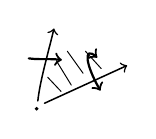
\begin{tikzpicture}[x=1cm,y=1cm,line cap=round,line join=round]
\fill (0,0) circle[radius=.025];
\draw[->,line width=.55pt] (.015,.10) .. controls (.04,.35) and (.16,.76) .. (.22,1.02);
\draw[->,line width=.55pt] (.10,.07)--(1.15,.55);
\draw[line width=.35pt] (.14,.40)--(.31,.22)
 (.25,.61)--(.44,.30)
 (.39,.73)--(.59,.45)
 (.62,.73)--(.82,.51);
\draw[->,line width=.8pt] (-.10,.64) .. controls (.03,.62) and (.14,.64) .. (.32,.62);
\draw[<->,line width=.8pt] (.77,.65) .. controls (.59,.80) and (.62,.56) .. (.81,.23);
\end{tikzpicture}}
) avec les relations génératrices
\[
(25)\qquad
\left\{\begin{aligned}
\unsure{(\sigma_0')^2}&=\unsure{(\sigma_1')^2}=\unsure{(\sigma_2')^2}
=\unsure{(\sigma_2'\sigma_0')^2}=1\\
\unsure{\bigl(\underbrace{\sigma_1'\sigma_0'}_{\rho_f}\bigr)^3}&=1
\end{aligned}\right.
\]

\margin{on pourrait aussi noter $\unsure{\sigma_\infty'}$ au lieu de $\unsure{\sigma_2'}$.
On aurait mieux fait de les noter \inserted{\unsure{ici}} carrément $r_0,r_1,r_\infty$ (au lieu de $\sigma_0,\sigma_1,\sigma_2$).}

Le sous-groupe \inserted{$\Pi_{0,3}'$} d'indice 2 \deleted{\illegible{1}}\inserted{(groupe cart. \unsure{triangul'} orienté)} est engendré par
\[
\unsure{\sigma_1'\sigma_0'}=\rho_f\inserted{\unsure{=\ell_\infty'}},\qquad
\unsure{\sigma_2'\sigma_1'}=\rho_s\inserted{\unsure{=\ell_0'}},\qquad
\unsure{\sigma_0'\sigma_2'}=\unsure{\sigma'|\sigma}\inserted{\unsure{=\ell_1'}},
\]
avec les relations génératrices
\[
(26)\qquad
\rho_f\sigma\rho_s\deleted{\unsure{\rho_s}}=1
\qquad
\sigma^2=\rho_f^3=1
\]
C'est donc le quotient de $\Pi_{0,3}$ par $\ell_1^2,\ell_\infty^3$
\[
(\unsure{27|17})\qquad
\left\{\begin{array}{rcl}
\Pi_{0,3}&\longrightarrow&\Pi_{0,3}'\\
\ell_0&\longmapsto&\ell_0'=\rho_s\\
\ell_1&\longmapsto&\ell_1'=\sigma\\
\ell_\infty&\longmapsto&\ell_\infty'=\rho_f
\end{array}\right.
\qquad,
\]
\deleted{\illegible{1}} Cet homomorphisme se prolonge en

\deleted{\unsure{(28)|(27)}}

\margin{89}
